\documentclass[fleqn, a4paper, 12pt, russian]{article}

\usepackage[utf8]{inputenc}
\usepackage[T1, T2A]{fontenc}
\usepackage[english, main = russian]{babel}
\usepackage{indentfirst}
\usepackage{graphicx}
\usepackage{natbib}
\usepackage{amsmath}
\usepackage{pdflscape}
\usepackage{caption, subcaption}
\graphicspath{{../imgs/}}

\captionsetup[figure]{name = Рисунок, labelsep = endash}
\captionsetup[table]{name = Таблица, labelsep = endash, justification=raggedright, singlelinecheck=false}
\setlength{\mathindent}{0pt}

\begin{document}

\begin{landscape}
	
$q = \begin{bmatrix} a(t)&x(t)&y(t) \end{bmatrix}$

$K = m( c_y\dot{a(t)}\cos a(t)  - \dot{x(t)} + c_x\dot{a(t)}\sin a(t)) (c_y\cos(a(t))\dot{a(t)} - \dot{x(t)} + c_x\sin(a(t))\dot{a(t)}) + (\dot{y(t)}) + c_x\dot{a(t)}\cos(a(t)) - c_y\dot{a(t)}\sin(a(t)))(\dot{y(t)} + c_x\cos(a(t))\dot{a(t)} - c_y\sin(a(t))\dot{a(t)})))/2 + (I\dot{a(t)}\dot{a(t)})/2$

$\frac{\partial K}{\partial q} = (\begin{array}{c} 0\\ 0\\ 0 \end{array})$

$\tiny{\frac{\partial K}{\partial \dot{q}}=\begin{bmatrix} I\,\dot{a(t)}-\frac{\mathrm{c_y}\,m\,\cos(a(t))\,\dot{x(t)}}{2}+\frac{\mathrm{c_x}\,m\,\cos(a(t))\,\dot{y(t)} (t)}{2}-\frac{\mathrm{c_x}\,m\,\sin(a(t))\,\dot{x(t)}}{2}-\frac{\mathrm{c_y}\,m\,\sin(a(t))\,\dot{y(t)}}{2}+{\mathrm{c_x}}^2\,m\,\cos(a(t))\,\dot{a(t)}+{\mathrm{c_y}}^2\,m\,\cos\textbf{a(t)}\,\dot{a(t)}-\frac{\mathrm{c_y}\,m\,\cos((a(t)))\,\dot{x(t)}}{2}+\frac{\mathrm{c_x}\,m\,\cos((a(t)))\,\dot{y(t)}}{2}-\frac{\mathrm{c_x}\,m\,\sin((a(t)))\,\dot{x(t)}}{2}-\frac{\mathrm{c_y}\,m\,\sin((a(t)))\,\dot{y(t)}}{2}\\ -\frac{m\,(\mathrm{c_y}\,\cos((a(t)))\,\dot{a(t)}-2\,\dot{x(t)}+\mathrm{c_x}\,\sin((a(t)))\,\dot{a(t)}+\mathrm{c_y}\,\cos(a(t))\,\dot{a(t)}+\mathrm{c_x}\,\sin(a(t))\,\dot{a(t)})}{2}\\ \frac{m\,(2\,\dot{y(t)}+\mathrm{c_x}\,\cos((a(t)))\,\dot{a(t)}-\mathrm{c_y}\,\sin((a(t)))\,\dot{a(t)}+\mathrm{c_x}\,\cos(a(t))\,\dot{a(t)}-\mathrm{c_y}\,\sin(a(t))\,\dot{a(t)})}{2} \end{bmatrix}}$

$\tiny{\frac{\partial}{\partial t}\frac{\partial K}{\partial \dot{q}}=\begin{bmatrix} I\,\ddot{a(t)}(t)-\frac{\mathrm{c_y}\,m\,\cos((a(t)))\,\ddot{x(t)}(t)}{2}+\frac{\mathrm{c_x}\,m\,\cos((a(t)))\,\ddot{y(t)}(t)}{2}-\frac{\mathrm{c_x}\,m\,\sin((a(t)))\,\ddot{x(t)}(t)}{2}-\frac{\mathrm{c_y}\,m\,\sin((a(t)))\,\ddot{y(t)}(t)}{2}-{\mathrm{c_x}}^2\,m\,{|\dot{a(t)}|}^2\,\sin(a(t))-{\mathrm{c_y}}^2\,m\,{|\dot{a(t)}|}^2\,\sin(a(t))-\frac{\mathrm{c_y}\,m\,\cos(a(t))\,\ddot{x(t)}(t)}{2}+\frac{\mathrm{c_x}\,m\,\cos(a(t))\,\ddot{y(t)}(t)}{2}-\frac{\mathrm{c_x}\,m\,\sin(a(t))\,\ddot{x(t)}(t)}{2}-\frac{\mathrm{c_y}\,m\,\sin(a(t))\,\ddot{y(t)}(t)}{2}+{\mathrm{c_x}}^2\,m\,\sin(a(t))\,{(\dot{a(t)})}^2+{\mathrm{c_y}}^2\,m\,\sin(a(t))\,{(\dot{a(t)})}^2+{\mathrm{c_x}}^2\,m\,\cos(a(t))\,\ddot{a(t)}(t)+{\mathrm{c_y}}^2\,m\,\cos(a(t))\,\ddot{a(t)}(t)-\frac{\mathrm{c_x}\,m\,(\dot{a(t)})\,\cos((a(t)))\,\dot{x(t)}}{2}-\frac{\mathrm{c_y}\,m\,(\dot{a(t)})\,\cos((a(t)))\,\dot{y(t)}}{2}+\frac{\mathrm{c_y}\,m\,(\dot{a(t)})\,\sin((a(t)))\,\dot{x(t)}}{2}-\frac{\mathrm{c_x}\,m\,(\dot{a(t)})\,\sin((a(t)))\,\dot{y(t)}}{2}-\frac{\mathrm{c_x}\,m\,\cos(a(t))\,\dot{a(t)}\,\dot{x(t)}}{2}-\frac{\mathrm{c_y}\,m\,\cos(a(t))\,\dot{a(t)}\,\dot{y(t)}}{2}+\frac{\mathrm{c_y}\,m\,\sin(a(t))\,\dot{a(t)}\,\dot{x(t)}}{2}-\frac{\mathrm{c_x}\,m\,\sin(a(t))\,\dot{y(t)}\,\dot{a(t)}}{2}\\ -\frac{m\,(\mathrm{c_x}\,\cos(a(t))\,{(\dot{a(t)})}^2-\mathrm{c_y}\,\sin(a(t))\,{(\dot{a(t)})}^2+\mathrm{c_y}\,\cos(a(t))\,\ddot{a(t)}(t)+\mathrm{c_x}\,\sin(a(t))\,\ddot{a(t)}(t)-2\,\ddot{x(t)}(t)+\mathrm{c_y}\,\cos((a(t)))\,\ddot{a(t)}(t)+\mathrm{c_x}\,\sin((a(t)))\,\ddot{a(t)}(t)+\mathrm{c_x}\,{|\dot{a(t)}|}^2\,\cos((a(t)))-\mathrm{c_y}\,{|\dot{a(t)}|}^2\,\sin((a(t))))}{2}\\ -\frac{m\,(\mathrm{c_y}\,\cos(a(t))\,{(\dot{a(t)})}^2+\mathrm{c_x}\,\sin(a(t))\,{(\dot{a(t)})}^2-\mathrm{c_x}\,\cos(a(t))\,\ddot{a(t)}(t)+\mathrm{c_y}\,\sin(a(t))\,\ddot{a(t)}(t)-2\,\ddot{y(t)}(t)-\mathrm{c_x}\,\cos((a(t)))\,\ddot{a(t)}(t)+\mathrm{c_y}\,\sin((a(t)))\,\ddot{a(t)}(t)+\mathrm{c_y}\,{|\dot{a(t)}|}^2\,\cos((a(t)))+\mathrm{c_x}\,{|\dot{a(t)}|}^2\,\sin((a(t))))}{2} \end{bmatrix}}$


$M(q)\begin{bmatrix}
	\ddot{a(t)}\\
	\ddot{x(t)}\\
	\ddot{y(t)}\\
\end{bmatrix}=\begin{bmatrix} -I\,\mathrm{\ddot{a(t)}}-\frac{m\,(2\,\mathrm{c_x}\,(\mathrm{\ddot{y(t)}}+\mathrm{c_x}\,\mathrm{\ddot{a(t)}})-2\,\mathrm{c_y}\,(\mathrm{\ddot{x(t)}}-\mathrm{c_y}\,\mathrm{\ddot{a(t)}}))}{2}\\ -m\,(\mathrm{\ddot{x(t)}}-\mathrm{c_y}\,\mathrm{\ddot{a(t)}})\\ -m\,(\mathrm{\ddot{y(t)}}+\mathrm{c_x}\,\mathrm{\ddot{a(t)}}) \end{bmatrix}$

$C\begin{bmatrix}
\dot{a(t)}\\
\dot{x(t)}\\
\dot{y(t)}\\
\end{bmatrix} = \begin{bmatrix} \mathrm{\dot{a(t)}}\,m\,(\mathrm{c_x}\,\mathrm{\dot{x(t)}}+\mathrm{c_y}\,\mathrm{\dot{y(t)}})\\ \mathrm{c_x}\,{\mathrm{\dot{a(t)}}}^2\,m\\ \mathrm{c_y}\,{\mathrm{\dot{a(t)}}}^2\,m \end{bmatrix}$

$G=(\begin{array}{c} 0\\ 0\\ 0 \end{array})$


$M(q) = \begin{bmatrix}
	-I-mc_x^2+c_y^2&-mc_y&mc_x\\
	mc_y&-m&0\\
	mc_x&0&-m\\
\end{bmatrix}$

$C(q)=\begin{bmatrix}
	0&\dot{a(t)}c_x&\dot{a(t)}c_y\\	
	\dot{a(t)}c_x&0&0\\
	\dot{a(t)}c_y&0&0\\
\end{bmatrix}$

$B(q) = \begin{bmatrix}
    (l+c_x)R&	(l-c_x)R\\
	R\cos(a)&	R\cos(a)\\
	R\sin(a)&	R\sin(a)\\
\end{bmatrix}$

$A = (\begin{bmatrix} 0 & 0 & 0 & 0 & 0 & 0\\ 0 & 0 & 0 & 0 & 0 & 0\\ 0 & 0 & 0 & 0 & 0 & 0\\ 0 & 0 & 0 & 0 & \frac{\mathrm{cx}\,\mathrm{dat}}{I+{\mathrm{cy}}^2\,m-{\mathrm{cy}}^2} & \frac{\mathrm{cy}\,\mathrm{dat}}{I+{\mathrm{cy}}^2\,m-{\mathrm{cy}}^2}\\ 0 & 0 & 0 & \frac{\mathrm{cx}\,\mathrm{dat}}{m} & \frac{\mathrm{cx}\,\mathrm{cy}\,\mathrm{dat}}{I+{\mathrm{cy}}^2\,m-{\mathrm{cy}}^2} & \frac{{\mathrm{cy}}^2\,\mathrm{dat}}{I+{\mathrm{cy}}^2\,m-{\mathrm{cy}}^2}\\ 0 & 0 & 0 & \frac{\mathrm{cy}\,\mathrm{dat}}{m} & \frac{{\mathrm{cx}}^2\,\mathrm{dat}}{I+{\mathrm{cy}}^2\,m-{\mathrm{cy}}^2} & \frac{\mathrm{cx}\,\mathrm{cy}\,\mathrm{dat}}{I+{\mathrm{cy}}^2\,m-{\mathrm{cy}}^2} \end{bmatrix})$



$B = (\begin{array}{ccc} 0 & 0 & 0\\ 0 & 0 & 0\\ 0 & 0 & 0\\ -\frac{1}{I+{\mathrm{cy}}^2\,m-{\mathrm{cy}}^2} & \frac{\mathrm{cy}}{I+{\mathrm{cy}}^2\,m-{\mathrm{cy}}^2} & -\frac{\mathrm{cx}}{I+{\mathrm{cy}}^2\,m-{\mathrm{cy}}^2}\\ -\frac{\mathrm{cy}}{I+{\mathrm{cy}}^2\,m-{\mathrm{cy}}^2} & -\frac{I-{\mathrm{cy}}^2}{m\,(I+{\mathrm{cy}}^2\,m-{\mathrm{cy}}^2)} & -\frac{\mathrm{cx}\,\mathrm{cy}}{I+{\mathrm{cy}}^2\,m-{\mathrm{cy}}^2}\\ -\frac{\mathrm{cx}}{I+{\mathrm{cy}}^2\,m-{\mathrm{cy}}^2} & \frac{\mathrm{cx}\,\mathrm{cy}}{I+{\mathrm{cy}}^2\,m-{\mathrm{cy}}^2} & -\frac{I+{\mathrm{cx}}^2\,m+{\mathrm{cy}}^2\,m-{\mathrm{cy}}^2}{m\,(I+{\mathrm{cy}}^2\,m-{\mathrm{cy}}^2)} \end{array})$



\begin{figure}[!h]
	\centering
	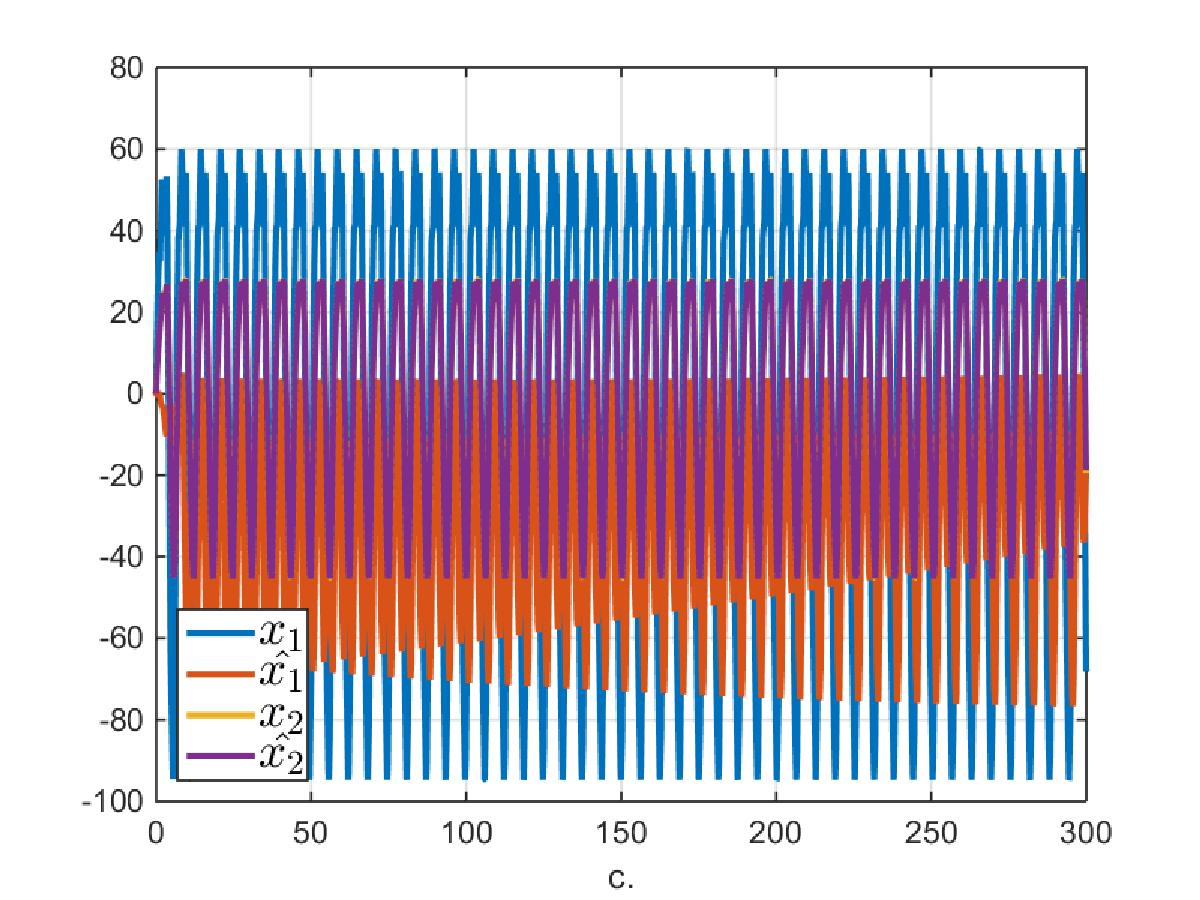
\includegraphics[width = 0.7\textwidth]{modeling62-x.jpg}
	\caption{Переменные состояния} 
	\label{modeling62-x}
\end{figure}

Тест привет

\end{landscape}
	
\end{document}